\begin{enumerate}
	\item L'administrateur se connecte au site avec ses identifiant. 
	\item Un nouveau bouton de navigation apparait dans la bar de navigation. 
	\item L'administrateur clique sur le bouton \textit{Admin}
	\item Il sélectionne \textit{Nouvelle Session} dans le menu déroulant. 
	\item L'administrateur atterris sur la page d'ajout de Sessions. 
	\item Il remplis le formulaire avec les bonne informations.
	\item Il clique sur \textit{Add}
\end{enumerate}

\newpage
\begin{figure}[h]
	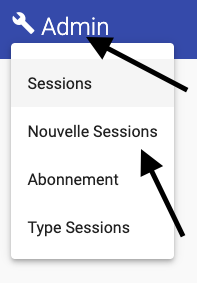
\includegraphics[width=0.4\textwidth,center]{Figures/us11-1}
	\caption{Bouton de navigation de l'administrateur}
\end{figure}

\vspace{\baselineskip}
\vspace{\baselineskip}
\begin{figure}[h]
	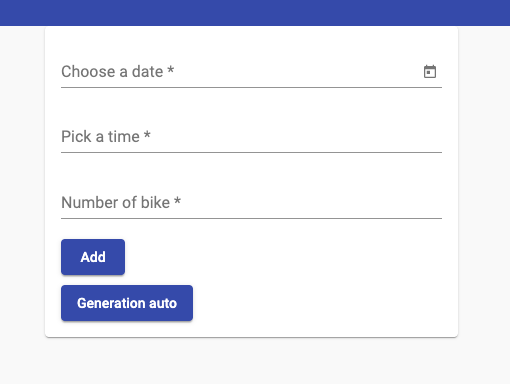
\includegraphics[width=0.5\textwidth,center]{Figures/us11-2}
	\caption{Bouton d'annulation de la session}
\end{figure}


\subsection{Gestion des erreurs}
	\begin{itemize}
		\item Tout les champs doivent être remplis, si ce n'est pas le cas il sera impossible d'envoyer le formulaire et l'administrateur aura une erreur afficher.
	\end{itemize}
	

\subsection{Diagramme de séquence}
	\begin{figure}[h]
		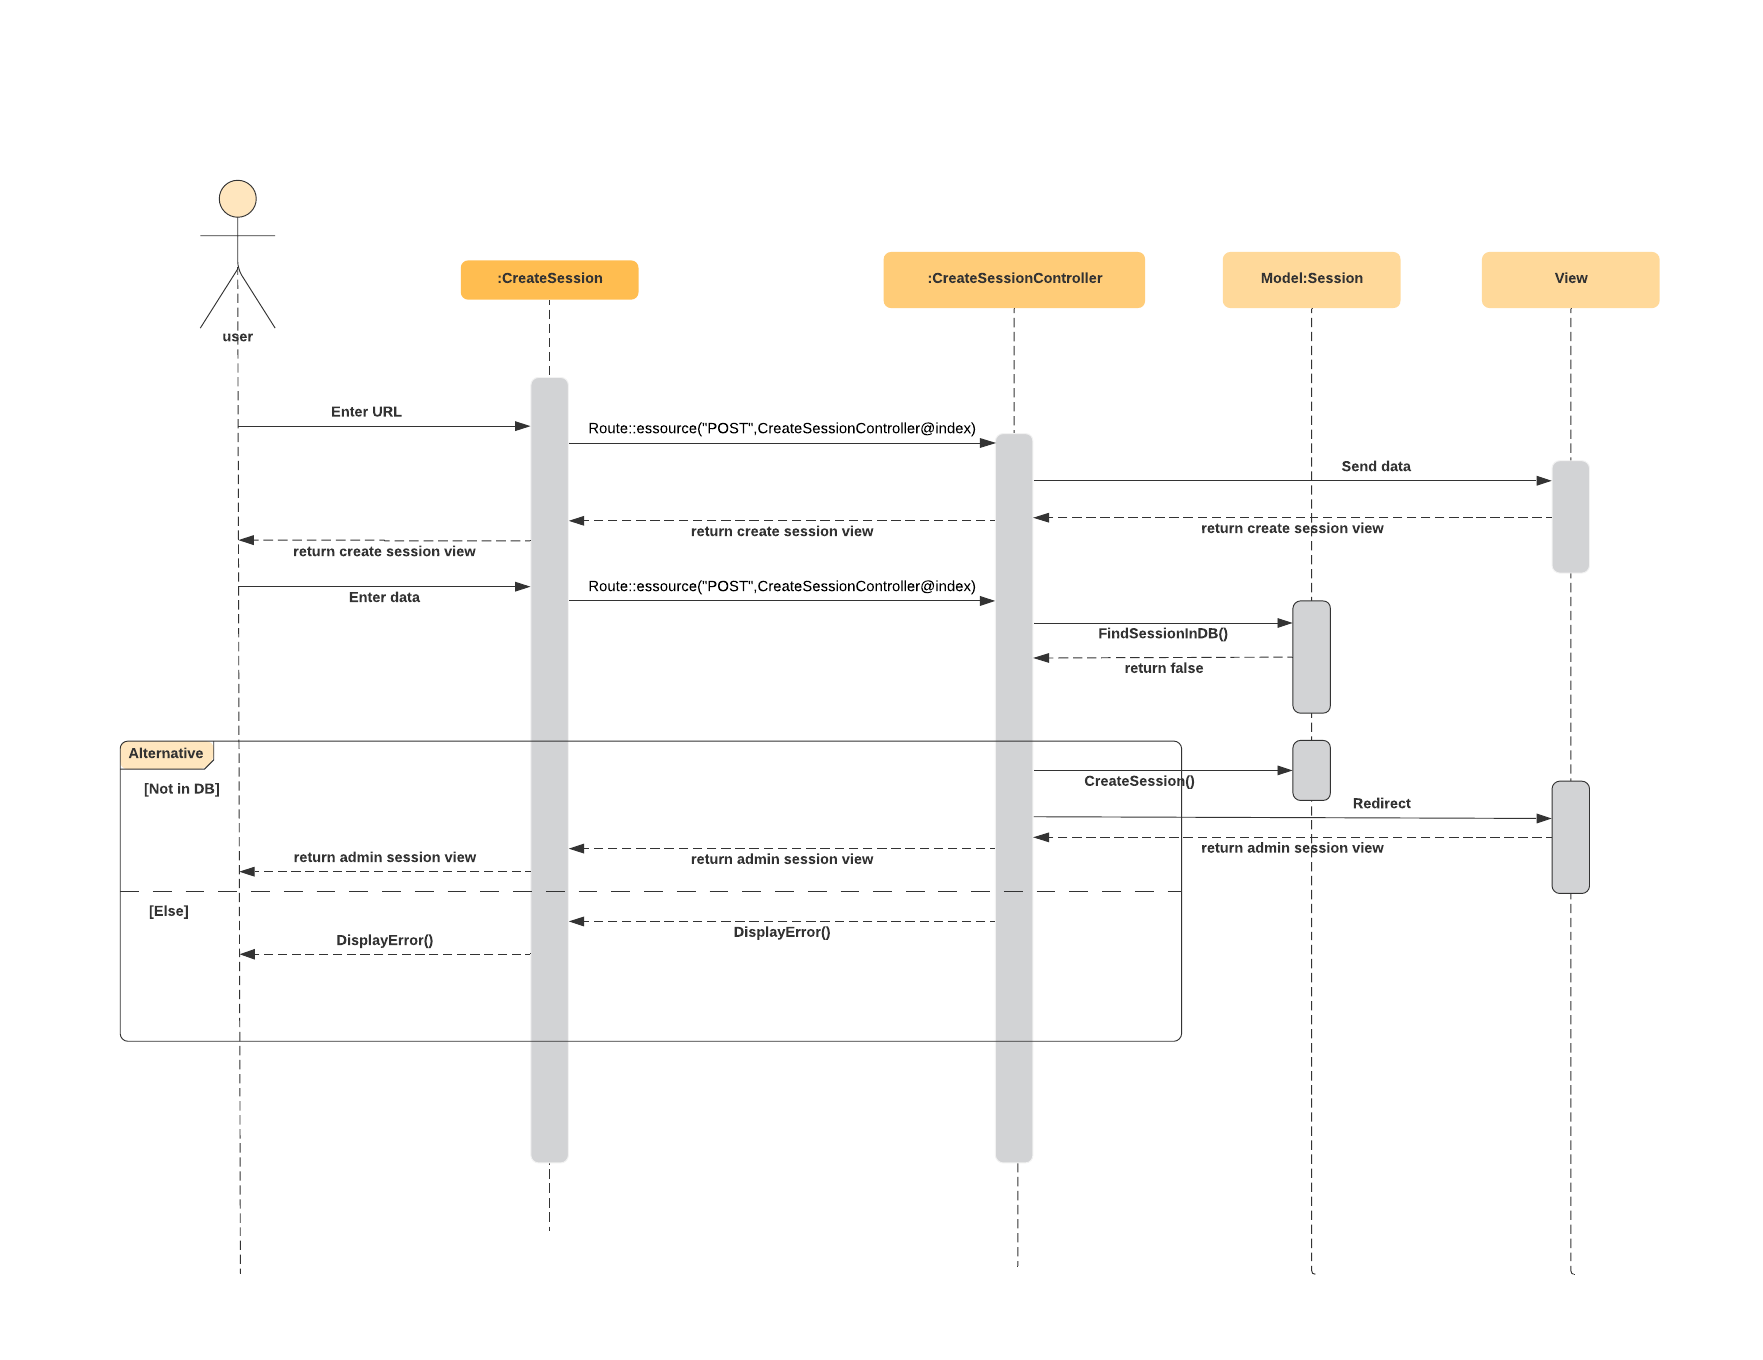
\includegraphics[width=\textwidth,center]{Diagramme/sequence-us11}
		\caption{Diagramme de séquence de l'ajout d'une session}
	\end{figure}
	
\subsection{Script concerné}
	\begin{itemize}
		\item \href{}{}
	\end{itemize}